\documentclass[xcolor=dvipsnames, xcolor=table]{beamer}
\usepackage[T1]{fontenc}
\usepackage[spanish,es-tabla]{babel}
\usepackage{amsmath}
\usepackage{amssymb,amsfonts,latexsym,cancel}
\usepackage{float}
\usepackage{graphicx}
\usepackage{epstopdf}
\usepackage{subfigure}
\usepackage[utf8]{inputenc}
\usepackage[dvipsnames]{xcolor}


\graphicspath{ {imagenes/} }
\definecolor{color1}{HTML}{23373B}
\definecolor{color2}{HTML}{2C4A52}
\definecolor{color3}{HTML}{EB811B}
\definecolor{color4}{HTML}{23373B}
\definecolor{color5}{HTML}{FFFFFF}

\setbeamercolor{frametitle}{fg=color5,bg=color4}
\setbeamertemplate{itemize item}{\color{color4}$\blacktriangleright$}

\title{Sistema de Información Integrado Para la Gestión de una Federación Sindical de Trabajadores}
\subtitle{CASO: Federación Sindical de Trabajadores de Entel S.A. (FesEntel)}
\author{Eddy Herrera Vargas}
\institute{IDS - USB}

\begin{document}

\begin{frame}

    \begin{figure}
      \begin{columns}
        \column{\dimexpr\linewidth-35mm-5mm}
        \column{3mm}
        \includegraphics[width=10mm]{usb.pdf}
      \end{columns}
    \end{figure}

  \vspace{-3mm}
  \Large\textbf{\textcolor{color1}{Sistema de Información Integrado Para la\\ Gestión de una Federación Sindical de Trabajadores}}\\
  \vspace{3mm}
  \small{\textcolor{color2}{\textbf{CASO:} Federación Sindical de Trabajadores de Entel S.A. (FesEntel)}}\\
  \vspace{2mm}
  \color{color3}{\rule{10.5cm}{0.6pt}}\\
  \vspace{8mm}
  \textcolor{color1}{\small{Eddy Herrera Vargas}\\
  \vspace{2mm}
  \scriptsize{IDS - USB }\\
  \vspace{2mm}
  \textit{\scriptsize{Noviembre, 2019}}}

\end{frame}

\begin{frame}
    \centering\color{color3}{\rule{7cm}{5pt}}\\
    \vspace{-3mm}
    \centering\color{color3}{\rule{7cm}{1.5pt}}\\
    \vspace{2mm}
    \centering\textbf{\huge{\textcolor{color1}{Generalidades}}}\\
    \centering\color{color3}{\rule{7cm}{1.5pt}}\\
\end{frame}

\begin{frame}
    \frametitle{Antecedentes}
    \begin{columns}
      \begin{column}{0.5\textwidth}
        \centering\textbf{\textcolor{color3}{Organización}}
        \vspace{3mm}
        \begin{itemize}
            \item Secretario Ejecutivo
            \item Secretario General
            \item Secretario de Relaciones
            \item Secretario de Finanzas
            \item Secretario de Organización
            \item Secretario de Conflictos
            \item Secretario Permanente
            \item Mensajero
         \end{itemize} 
      \end{column}
      \begin{column}{0.5\textwidth} 
        \centering\textbf{\textcolor{color3}{Misión de la\\Institución}}\\
        \vspace{6mm}
        \scriptsize Defender los derechos fundamentales de los trabajadores afiliados, consagrados
por la Constitución Política del Estado, la Ley General del Trabajo (LGT), la
Declaración Universal de los Derechos Humanos y otros: defendiendo de esta
manera los intereses materiales, la integridad moral de la persona humana, la
justicia y libertad en todas sus formas de los trabajadores, oponiéndose a toda
explotación inhumana de sus afiliados.
      \end{column}
    \end{columns}
\end{frame}

\begin{frame}
    \frametitle{Descripción del Problema}
    
    \begin{columns}
      \begin{column}{0.3\textwidth}
        \centering\textbf{\textcolor{color3}{Manejo de Correspondencia}\vspace{3mm}}
        \vspace{10mm}
        \includegraphics[width=20mm]{002-delivery-man.pdf}
      \end{column}
      \begin{column}{0.3\textwidth}
        \centering\textbf{\textcolor{color3}{Registro de Afiliados}\vspace{3mm}}
        \vspace{10mm}
        \includegraphics[width=20mm]{010-affiliate.pdf}
      \end{column}
      \begin{column}{0.3\textwidth}
        \centering\textbf{\textcolor{color3}{Estatutos y Normas}\vspace{3mm}}
        \vspace{10mm}
        
\includegraphics[width=20mm]{004-auction.pdf}
      \end{column}
    \end{columns}
    \begin{columns}
      \begin{column}{0.5\textwidth}
        \centering\textbf{\textcolor{color3}{Administración\\ de Información}\vspace{3mm}}
        \\
        
\includegraphics[width=20mm]{007-information.pdf}
      \end{column}
      \begin{column}{0.5\textwidth}
        \centering\textbf{\textcolor{color3}{Federaciones\\ y Sindicatos}\vspace{3mm}}
        \\
        
\includegraphics[width=20mm]{005-union.pdf}
      \end{column}
    \end{columns}
\end{frame}

\begin{frame}
    \frametitle{Problema Principal}
    \large\centering Los procedimientos para difusión de información, el manejo económico, el manejo de la información sobre otros recursos con los que cuenta la institución, la gestión de la información de los afiliados, son realizados de manera empírica y en hojas de cálculo, lo que conlleva a la desinformación sobre la gestión que se esta realizando en la institución, la dificultad para la elaboración de informes sobre estados financieros y otros, la perdida y acceso dificultoso a la información, también el desconocimiento por parte del afiliado respecto a sus derechos y deberes dentro la LGT y otros estatutos y normas que afecten sus intereses.
\end{frame}

\begin{frame}
    \frametitle{Problemas Secundarios}
    \vspace{5mm}
    \begin{columns}
      \begin{column}{0.3\textwidth}
        \centering\textbf{\textcolor{color3}{\small Inadecuada Difusión de Información}\vspace{3mm}}
        \vspace{10mm}
        \includegraphics[width=20mm]{022-news.pdf}
      \end{column}
      \begin{column}{0.3\textwidth}
        \centering\textbf{\textcolor{color3}{\small Informes Financieros Erróneos}\vspace{3mm}}
        \vspace{10mm}
        \includegraphics[width=20mm]{018-money-1}
      \end{column}
      \begin{column}{0.3\textwidth}
        \centering\textbf{\textcolor{color3}{\small Pérdida de Documentación}\vspace{3mm}}
        \vspace{10mm}
        
\includegraphics[width=20mm]{023-document}
      \end{column}
    \end{columns}
    \vspace{-2mm}
    \begin{columns}
      \begin{column}{0.3\textwidth}
        \centering\textbf{\textcolor{color3}{\small Difícil Acceso a Información}\vspace{3mm}}
        \vspace{10mm}
        \includegraphics[width=20mm]{028-paper}
      \end{column}
      \begin{column}{0.3\textwidth}
        \centering\textbf{\textcolor{color3}{\small Afiliados\\Disconformes}\vspace{3mm}}
        \vspace{10mm}
        
\includegraphics[width=20mm]{032-anger}
      \end{column}
      \begin{column}{0.3\textwidth}
        \centering\textbf{\textcolor{color3}{\small Pérdida de Bienes Muebles}\vspace{3mm}}
        \vspace{10mm}
        \includegraphics[width=20mm]{029-lost-items}
      \end{column}      
    \end{columns}
\end{frame}

\begin{frame}
    \frametitle{Objetivo General}
 
  \centering\large Desarrollar un sistema de información integrado para la gestión de una federación
sindical de trabajadores: que permita la administración de la información de
los afiliados a FesEntel, el registro de correspondencia remitida como recibida,
la administración de documentación digitalizada, el registro de los bienes
que posee la institución, la administración contable y la difusión información
o documentación a través de un sitio web; que asegure la integridad, el
manejo adecuado de la información, realizando informes financieros correctos
y oportunos, además mantenga informado a los afiliados a FesEntel.

\end{frame}

\begin{frame}
    \frametitle{Objetivos Específicos}
    \vspace{3mm}
    \begin{columns}
      \begin{column}{0.3\textwidth}
        \centering\textbf{\textcolor{color3}{\small Compartir Información y Documentación}\vspace{3mm}}
        \vspace{10mm}
        \includegraphics[width=20mm]{033-laptop}
      \end{column}
      \begin{column}{0.3\textwidth}
        \centering\textbf{\textcolor{color3}{\small Automatizar Registro de\\Flujo de Caja}\vspace{3mm}}
        \vspace{10mm}
        
\includegraphics[width=20mm]{019-coin}
      \end{column}
      \begin{column}{0.3\textwidth}
        \centering\textbf{\textcolor{color3}{\small Automatizar Registro de Afiliados}\vspace{3mm}}
        \vspace{10mm}
        \includegraphics[width=20mm]{laptop}
      \end{column}
    \end{columns}
    \vspace{-5mm}
    \begin{columns}
      \begin{column}{0.3\textwidth}
        \centering\textbf{\textcolor{color3}{\small Centralizar Información de Correspondencia}\vspace{3mm}}
        \vspace{10mm}
        
\includegraphics[width=20mm]{036-system}
      \end{column}
      \begin{column}{0.3\textwidth}
        \centering\textbf{\textcolor{color3}{\small Resguardar Documentación Digitalizándola}\vspace{3mm}}
        \vspace{10mm}
        \includegraphics[width=20mm]{035-monitor}
      \end{column}
      \begin{column}{0.3\textwidth}
        \centering\textbf{\textcolor{color3}{\small Concentrar\\Registro de Bienes Muebles}\vspace{3mm}}
        \vspace{10mm}
        \includegraphics[width=20mm]{031-house}
      \end{column}      
    \end{columns}
\end{frame}

\begin{frame}
    \frametitle{Justificación}
    \vspace{5mm}
    \begin{columns}
      \begin{column}{0.5\textwidth}
        \centering\textbf{\textcolor{color3}{Social}\vspace{3mm}}\\
        \vspace{2mm}
        \includegraphics[width=20mm]{global}
      \end{column}
      \begin{column}{0.5\textwidth}
        \centering\textbf{\textcolor{color3}{Técnica}\vspace{3mm}}\\
        \vspace{2mm}
        \includegraphics[width=20mm]{tecnica}
      \end{column}
    \end{columns}
    \vspace{-2mm}
    \begin{columns}
      \begin{column}{1\textwidth}
        \centering\textbf{\textcolor{color3}{Operativa}\vspace{3mm}}\\
        \vspace{2mm}
        \includegraphics[width=20mm]{local-area}
      \end{column}
    \end{columns}
\end{frame}

\begin{frame}
    \frametitle{Alcances}
        \vspace{5mm}
    \begin{columns}
      \begin{column}{0.3\textwidth}
        \centering\textbf{\textcolor{color3}{\small Manejador de Contenidos}\vspace{3mm}}
        \vspace{10mm}
        \includegraphics[width=20mm]{002-monitor}
      \end{column}
      \begin{column}{0.3\textwidth}
        \centering\textbf{\textcolor{color3}{\small Contabilidad Básica}\vspace{3mm}}
        \vspace{10mm}
        \includegraphics[width=20mm]{001-accounting}
      \end{column}
      \begin{column}{0.3\textwidth}
        \centering\textbf{\textcolor{color3}{\small Afiliación de Empleados}\vspace{3mm}}
        \vspace{10mm}
        \includegraphics[width=20mm]{003-affiliate}
      \end{column}
    \end{columns}
    \vspace{-2mm}
    \begin{columns}
      \begin{column}{0.3\textwidth}
        \centering\textbf{\textcolor{color3}{\small Manejo de Correspondencia}\vspace{3mm}}
        \vspace{10mm}
        \includegraphics[width=20mm]{026-message}
      \end{column}
      \begin{column}{0.3\textwidth}
        \centering\textbf{\textcolor{color3}{\small Archivo de Documentos}\vspace{3mm}}
        \vspace{10mm}
        \includegraphics[width=20mm]{003-file}
      \end{column}
      \begin{column}{0.3\textwidth}
        \centering\textbf{\textcolor{color3}{\small Control de Bienes Muebles}\vspace{3mm}}
        \vspace{10mm}
        
\includegraphics[width=20mm]{004-armchair}
      \end{column}      
    \end{columns}
\end{frame}

\begin{frame}
    \frametitle{Límites}
    \begin{columns}
      \begin{column}{0.5\textwidth}
        \centering\textbf{\textcolor{color3}{No realiza contabilidad Avanzada}\vspace{3mm}}\\
        \vspace{5mm}
        \includegraphics[width=20mm]{contabilidad}
      \end{column}
      \begin{column}{0.5\textwidth}
        \centering\textbf{\textcolor{color3}{Puede no adaptarse a toda federación de trabajadores}\vspace{3mm}}\\
        \vspace{5mm}
        \includegraphics[width=20mm]{error}
      \end{column}
    \end{columns}
\end{frame}

\begin{frame}
    \centering\color{color3}{\rule{10cm}{5pt}}\\
    \vspace{-3mm}
    \centering\color{color3}{\rule{10cm}{1.5pt}}\\
    \vspace{2mm}
    \centering\textbf{\huge{\textcolor{color1}{Factibilidad y Estimación\\ de Costos}}}\\
    \centering\color{color3}{\rule{10cm}{1.5pt}}\\
\end{frame}

\begin{frame}
    \frametitle{COCOMO II}
    \centering\textbf{\textcolor{color3}{Para la estimación de esfuerzo requerido\\se utilizó la fórmula:}}

\[PM_{estimado} = PM_{nominal} * \prod_{i=1}^{7}EM_{i}\]
\[PM_{nominal} = A * (KSLOC)^{B}\]
\[B = 1.01 + 0.01 * \sum_{j=1}^{5}Wj\]
\end{frame}

\begin{frame}
    \frametitle{Costos del Proyecto}

    \begin{columns}
      \begin{column}{0.3\textwidth}
        \centering\textbf{\textcolor{color3}{\small Tiempo Requerido}\vspace{2mm}}
        \tiny\[TDEV_{estimado} = 10.86\]
      \end{column}
      \begin{column}{0.3\textwidth}
        \centering\textbf{\textcolor{color3}{\small Personal Estimado}\vspace{2mm}}
        \tiny\[STAFF_{estimado} = 2.79\]
      \end{column}
      \begin{column}{0.3\textwidth}
        \centering\textbf{\textcolor{color3}{\small Costo Estimado}\vspace{2mm}}
        \tiny\[Costo_{estimado} = 60529.77 Bs\]
      \end{column}
    \end{columns}

    \vspace{5mm}
    \centering\textbf{\textcolor{color3}{\small Costo estimado del sistema}\vspace{2mm}}
    \renewcommand{\arraystretch}{1.1}
    \begin{table}[]
    \begin{tabular}{|l|l|}
    \hline
    \multicolumn{1}{|c|}{\textbf{\tiny Detalle}} & \multicolumn{1}{c|}{\textbf{\tiny Costo}} \\ \hline
    \textbf{\tiny Costo estimado de los elementos técnicos} &\\\hline
    \quad \tiny Hardware & \tiny 4833 Bs  \\ \hline
    \quad \tiny Software & \tiny 0 Bs \\ \hline
    \textbf{\tiny Costo estimado del desarrollo del software} & \tiny 60500 Bs \\ \hline
    \multicolumn{1}{|r|}{\textbf{\tiny Total}} & \cellcolor[HTML]{FFCCC9}\textbf{\tiny 65333 Bs} \\ \hline
    \end{tabular}
    \end{table}

\end{frame}

\begin{frame}
    \centering\color{color3}{\rule{10cm}{5pt}}\\
    \vspace{-3mm}
    \centering\color{color3}{\rule{10cm}{1.5pt}}\\
    \vspace{2mm}
    \centering\textbf{\huge{\textcolor{color1}{Ingeniaría del Proyecto}}}\\
    \centering\color{color3}{\rule{10cm}{1.5pt}}\\
\end{frame}

\begin{frame}
    \frametitle{Proceso Ágil Unificado}
    \centering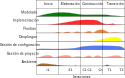
\includegraphics[width=9.5cm]{aup}
\end{frame}

\begin{frame}
    \frametitle{\textit{Fase de Inicio:} Modelo de requerimientos}
    \begin{columns}
      \begin{column}{0.4\textwidth}
        \centering\textbf{\textcolor{color3}{\small Caso de uso general\\ del modelo de negocio}\vspace{2mm}}
        \centering\includegraphics[width=5cm]{CUgeneral}
      \end{column}
      \begin{column}{0.6\textwidth}
        \centering\textbf{\textcolor{color3}{\small Modelo de negocio,\\ manejador de contenidos}\vspace{6mm}}
        \includegraphics[width=6cm]{CUcms}
      \end{column}
    \end{columns}
\end{frame}

\begin{frame}
    \frametitle{\textit{Fase de Inicio:} Modelo de requerimientos}
    \begin{columns}
      \begin{column}{0.5\textwidth}
        \centering\textbf{\textcolor{color3}{\small Modelo de negocio,\\ contabilidad}\vspace{5mm}}
        \centering\includegraphics[width=5cm]{CUcon}
      \end{column}
      \begin{column}{0.5\textwidth}
        \centering\textbf{\textcolor{color3}{\small Modelo de negocio,\\bien mueble}\vspace{5mm}}
        \includegraphics[width=5.5cm]{CUbm}
      \end{column}
    \end{columns}
\end{frame}

\begin{frame}
    \frametitle{\textit{Fase de Inicio:} Modelo de requerimientos}
    \begin{columns}
      \begin{column}{0.45\textwidth}
        \centering\textbf{\textcolor{color3}{\small Modelo de negocio,\\ correspondencia}\vspace{4mm}}
        \centering\includegraphics[width=5.3cm]{CUcorr}
      \end{column}
      \begin{column}{0.55\textwidth}
        \centering\textbf{\textcolor{color3}{\small Modelo de negocio,\\archivo}\vspace{4mm}}
        \includegraphics[width=6cm]{CUarc}
      \end{column}
    \end{columns}
\end{frame}

\begin{frame}
    \frametitle{\textit{Fase de Inicio:} Modelo de requerimientos}
         \centering\textbf{\textcolor{color3}{\small Modelo de negocio,\\ afiliados}\vspace{2mm}}
        \centering\includegraphics[width=10cm]{CUafl}
\end{frame}

\begin{frame}
    \frametitle{\textit{Fase de Elaboración:} Modelo de Datos}
    \centering\includegraphics[width=6.5cm]{clasesd}
\end{frame}

\begin{frame}
    \frametitle{\textit{Fase de Elaboración:} Modelo de Despliegue}
    \centering\includegraphics[width=7.5cm]{des}
\end{frame}

\begin{frame}
    \frametitle{\textit{Fase de Construcción:} Interfaces}
    \begin{columns}
      \begin{column}{0.5\textwidth}
        \centering\textbf{\textcolor{color3}{ Diseño Responsivo}\vspace{6mm}}
        \centering\includegraphics[width=3.5cm]{responsive}
      \end{column}
      \begin{column}{0.5\textwidth}
        \centering\textbf{\textcolor{color3}{ Interfaz de Usuario}\vspace{6mm}}
        \includegraphics[width=3.5cm]{ui}
      \end{column}
    \end{columns}
\end{frame}

\begin{frame}
    \frametitle{\textit{Fase de Transición:} Pruebas}
    \begin{columns}
      \begin{column}{0.5\textwidth}

        \centering\includegraphics[width=4.5cm]{testing}
      \end{column}
      \begin{column}{0.5\textwidth}
        \centering\textbf{{\small Las pruebas de software consisten en la dinámica de la verificación del comportamiento de un programa en un conjunto finito de casos de prueba, debidamente seleccionados de por lo general infinitas ejecuciones de dominio, contra la del comportamiento esperado.\textit{(Ecured})}\vspace{2mm}}
      \end{column}
    \end{columns}
\end{frame}

\begin{frame}
    \frametitle{\textit{Fase de Transición:} Pruebas de caja blanca y negra}
    \begin{columns}
      \begin{column}{0.5\textwidth}
        \centering\textbf{\textcolor{color3}{\small Prueba de\\Caja Blanca}\vspace{5mm}}
        \centering\includegraphics[width=5cm]{CBlanca}
      \end{column}
      \begin{column}{0.5\textwidth}
        \centering\textbf{\textcolor{color3}{\small Prueba de\\Caja Negra}\vspace{5mm}}
        \centering\includegraphics[width=5cm]{CNegra}
      \end{column}
    \end{columns}
\end{frame}

\begin{frame}
    \frametitle{\textit{Fase de Transición:} Calidad}
    \begin{columns}
      \begin{column}{0.7\textwidth}

        \centering\includegraphics[width=6.5cm]{mccall}
      \end{column}
      \begin{column}{0.3\textwidth}
        \textbf{\textcolor{color3}{\small Modelo Mccall}\vspace{2mm}}
        \small\quad Mantenimiento
        \quad Flexibilidad
        \vspace{2mm}
        Susceptibilidad
        \quad Portabilidad
        \quad Reusabilidad
        \vspace{2mm}
        Interoperabilidad
        \quad Correción
        \quad Confiabilidad
        \quad Eficiencia
        \quad Usabilidad0
        \quad Integradad
      \end{column}
    \end{columns}
\end{frame}

\begin{frame}
    \frametitle{Conclusiones}
    \vspace{-2mm}
    \begin{columns}
      \begin{column}{0.4\textwidth}
        
        \centering\includegraphics[width=3.5cm]{center}
      \end{column}
      \begin{column}{0.6\textwidth}
        
        \centering\includegraphics[width=5.5cm]{crud}
      \end{column}
      
    \end{columns}
    \begin{columns}
      
      \begin{column}{1\textwidth}
        
\centering\includegraphics[width=5cm]{desarrollo}
      \end{column}
    \end{columns}
\end{frame}


\begin{frame}
    \frametitle{Recomendaciones}
    \begin{columns}
      \begin{column}{0.5\textwidth}
        \centering\textbf{\textcolor{color3}{\small Seguridad}}\\
        \vspace{3mm}
        \centering\includegraphics[width=2cm]{001-privacy}
      \end{column}
      \begin{column}{0.5\textwidth}
        \centering\textbf{\textcolor{color3}{\small Backup}}\\
        \vspace{3mm}
        \centering
\includegraphics[width=2cm]{002-backup}
      \end{column}
      
    \end{columns}
    \vspace{5mm}
    \begin{columns}
      \begin{column}{0.5\textwidth}
        \centering\textbf{\textcolor{color3}{\small Mantenimiento}}\\
        \vspace{3mm}
        \centering\includegraphics[width=2cm]{003-optimize}
      \end{column}
      \begin{column}{0.5\textwidth}
        \centering\textbf{\textcolor{color3}{\small Familiarización}}\\
        \vspace{3mm}
        \centering\includegraphics[width=2cm]{working}
      \end{column}
      
    \end{columns}
\end{frame}

\begin{frame}
    \centering\textbf{\huge{\textcolor{color1}{MUCHAS GRACIAS}}}    
\end{frame}

\end{document}
